\documentclass[12pt,a4paper]{report}
\usepackage[utf8]{inputenc}
\usepackage[spanish]{babel}

\usepackage[usenames, dvipsnames]{color}

%adjust your page margins here
\usepackage[top=0.70in, bottom=0.70in, left=0.8in,right=0.80in]{geometry} % setting the page alignment with this package
\usepackage[pdftex]{graphicx} %for embedding images
\usepackage[%dvips, % commented for pdflatex
bookmarks,  colorlinks=false]{hyperref} %for creating links in the pdf version and other additional pdf attributes, no effect on the printed document
\hypersetup{%
    pdfborder = {0 0 0}
}
\usepackage[final]{pdfpages} %for embedding another pdf, remove if not required
\usepackage{float} %used for figure placement with H as a parameter
\usepackage{hyperref}

%% Paquete para referencias de APA
%% Importante: Debe incluirse después de hyperref
\usepackage[]{apacite}

\usepackage{pslatex} % for times new roman, old package, but works
\usepackage{array} % for making text bold in table
\usepackage{setspace}
\usepackage{float}
\usepackage{enumerate}
\usepackage{longtable}
\usepackage{amssymb}

\usepackage[font=small,labelfont=bf]{caption}
\def\figurename{\textbf{Figure }}

\usepackage{listings}

\definecolor{dkgreen}{rgb}{0,0.6,0}
\definecolor{gray}{rgb}{0.5,0.5,0.5}
\definecolor{mauve}{rgb}{0.58,0,0.82}
 
\lstset{ %
  language=Java,                % the language of the code
  basicstyle=\footnotesize,           % the size of the fonts that are used for the code
  numbers=left,                   % where to put the line-numbers
  numberstyle=\tiny\color{gray},  % the style that is used for the line-numbers
  stepnumber=1,                   % each line is numbered
  numbersep=5pt,                  % how far the line-numbers are from the code
  backgroundcolor=\color{white},      % choose the background color. You must add \usepackage{color}
  showspaces=false,               % show spaces adding particular underscores
  showstringspaces=false,         % underline spaces within strings
  showtabs=false,                 % show tabs within strings adding particular underscores
  frame=single,                   % adds a frame around the code
  rulecolor=\color{black},        % if not set, the frame-color may be changed on line-breaks within not-black text (e.g. commens (green here))
  tabsize=2,                      % sets default tabsize to 2 spaces
  captionpos=b,                   % sets the caption-position to bottom
  breaklines=true,                % sets automatic line breaking
  breakatwhitespace=false,        % sets if automatic breaks should only happen at whitespace
  title=\lstname,                   % show the filename of files included with \lstinputlisting;
                                  % also try caption instead of title
  keywordstyle=\color{blue},          % keyword style
  commentstyle=\color{dkgreen},       % comment style
  stringstyle=\color{mauve},         % string literal style
  escapeinside={\%*}{*)},            % if you want to add a comment within your code
  morekeywords={*,...}               % if you want to add more keywords to the set
}

%For the header and footer
\usepackage{fancyhdr}
\fancypagestyle{plain}{%
\fancyfoot[L]{\emph{Escuela de Ingeniería en Computación, ITCR, Alajuela}} % except the center
\fancyfoot[R]{\thepage}
\renewcommand{\headrulewidth}{0.4pt}
\renewcommand{\footrulewidth}{0.4pt}
}

\pagestyle{fancy}

\rhead{\emph{NAME OF PROJECT}}

\fancyfoot[LO,LE]{\emph{Escuela de Ingeniería en Computación, ITCR, Alajuela}}
\cfoot{}
\fancyfoot[RO, RE]{\thepage}
\renewcommand{\headrulewidth}{0.4pt}
\renewcommand{\footrulewidth}{0.4pt}
%For the header and footer Over

%Page Border
\usepackage{pgf}
\usepackage{pgfpages}

\pgfpagesdeclarelayout{boxed}
{
  \edef\pgfpageoptionborder{0pt}
}
{
  \pgfpagesphysicalpageoptions
  {%
    logical pages=1,%
  }
  \pgfpageslogicalpageoptions{1}
  {
    border code=\pgfsetlinewidth{2pt}\pgfstroke,%
    border shrink=\pgfpageoptionborder,%
    resized width=.95\pgfphysicalwidth,%
    resized height=.95\pgfphysicalheight,%
    center=\pgfpoint{.5\pgfphysicalwidth}{.5\pgfphysicalheight}%
  }%
}
\pgfpagesuselayout{boxed}
\setlength{\parindent}{1cm}
%GLOBAL SETTINGS OVER, DOCUMENT BEGINS
\begin{document}
\renewcommand\bibname{Referencias bibliográficas}
\lhead{ }

%FROM HERE YOUR PAGES START GETTING ADDED

% includes the cover page
\newpage
\begin{center}
\thispagestyle{empty}

\includegraphics[scale=1]{project/images/Firma-TEC.png}\\
\vspace{1cm}
\Large{\textbf{INFORME DE AVANCE\\ \large{DEL PROYECTO}}}\\[0.7cm]
\LARGE{\textsc {\textbf{``NOMBRE DEL PROYECTO''}}}\\[0.5cm]
\Large{\textbf{\\Para el curso de}}
\LARGE{\textbf{\\PROYECTO DE INGENIERÍA DE SOFTWARE\\}}
\vspace{0.5cm}
\Large{\textbf{\\CAMPUS TECNOLÓGICO DE SAN JOSÉ\\ESCUELA DE INGENIERÍA EN COMPUTACIÓN\\BACHILLERATO EN INGENIERÍA EN COMPUTACIÓN\\PLAN 410\\}}
\vspace{1cm}
\Large{\textbf{\\EQUIPO DE TRABAJO}}\\[0.3cm]
\begin{table}[h]
\centering
\large{
\begin{tabular}{>{\bfseries}lc>{\bfseries}r}
NOMBRE COMPLETO & & COORDINADOR\\ %SCRUM MASTER
NOMBRE COMPLETO & & DESARROLLADOR\\
NOMBRE COMPLETO & & DESARROLLADOR\\
NOMBRE COMPLETO & & DESARROLLADOR\\
 & & \\
NOMBRE COMPLETO & & SUPERVISOR\\ %PRODUCT OWNER O CLIENTE
\end{tabular}}
\end{table}
\vspace{0.5cm}
\large{\textbf{BAJO LA SUPERVISIÓN DE}}\\
\large{\textbf{RODOLFO MORA ZAMORA}}\\
\vspace{1cm}
\large{\textbf{SAN JOSÉ}}
\large{\textbf{\\2019}}\\
\vspace{1cm}
\newpage
\end{center}
\newpage

\begin{center}
\thispagestyle{empty}
\vspace{2cm}
\LARGE{\textbf{RESUMEN}}\\[1.0cm]
\end{center}
\thispagestyle{empty}
Lorem ipsum dolor sit amet, consectetur adipiscing elit. Integer at posuere mi. Nulla ipsum sem, sagittis a leo et, mollis malesuada mauris. Donec id urna vel ipsum imperdiet elementum at at orci. Etiam commodo nulla nec metus consectetur, vitae pulvinar libero sodales. Morbi eget faucibus risus. Nam mauris purus, placerat pulvinar est eget, laoreet tempus magna. Integer ultricies in justo a dictum. Praesent at varius urna. Donec tristique, ante id egestas rutrum, odio felis mollis ante, ac bibendum nisi metus vel mauris. Phasellus blandit odio ut magna tincidunt tincidunt.

Integer sodales nisl at leo fermentum, sit amet accumsan enim semper. Phasellus laoreet dignissim arcu a vehicula. Nam id vehicula eros, vitae venenatis erat. Integer lacinia arcu quis nisl faucibus congue. Pellentesque interdum a magna vel consequat. Suspendisse potenti. Donec blandit sapien at arcu suscipit, eu congue magna pharetra. Curabitur mattis, lectus et posuere dictum, lectus ligula malesuada magna, sit amet egestas est dolor id lorem. Donec id gravida magna, nec vestibulum tortor. Duis quis varius nisi. Sed fringilla nisl eget ex mollis ornare. Proin tempor, justo eget iaculis blandit, felis enim faucibus justo, ac tincidunt neque erat quis neque. Donec vitae tempor ex. Sed ut augue sit amet mauris mollis ultrices at sit amet erat. \\
\textbf{Palabras clave: }keyword1, keyword2 % adds the abstract page
\newpage

%TABLE OF CONTENTS AND LIST OF FIGURES ARE AUTOMATICALLY ADDED BY FOLLOWING COMMANDS
%ADD FIGURE OF TABLES IF YOU NEED TO, CHECK DOCUMENTATION
\pagenumbering{roman} %numbering before main content starts


%To reset the Header & Footer for TOC and LOF
\pagestyle{empty}
\addtocontents{toc}{\protect\thispagestyle{empty}}
\tableofcontents % adds Index Page

\addtocontents{lof}{\protect\thispagestyle{empty}}
\listoffigures % adds List of Figures
\cleardoublepage

%And reset back the settings we choose for Header and Footer
\pagestyle{fancy}

\newpage
\pagenumbering{arabic} %reset numbering to normal for the main content

\chapter{Introducción}
\section{Descripción del proyecto}
\subsection{Antecedentes}
Incluya en esta sección una reseña histórica del proyecto 
\subsection{Objetivos}
Liste los objetivos del proyecto.
\begin{itemize}
    \item \textbf{Objetivo General}
    \begin{itemize}
        \item Objetivo general del proyecto redactado con un verbo infinitivo. Debe cubrir las generalidades del proyecto
    \end{itemize}
    \item \textbf{Objetivos Específicos}
    \begin{itemize}
        \item Objetivos específicos con mayor nivel de detalle
        \item Normalmente los objetivos específicos hacen referencia a "módulos" del sistema
    \end{itemize}
\end{itemize}
\section{Datos gerenciales del proyecto}
\subsection{Acta Constitutiva del proyecto}
Lorem ipsum dolor sit amet, consectetur adipiscing elit. Nunc sed cursus dolor. Aliquam mi ipsum, ullamcorper ac tellus iaculis, interdum egestas orci. In vitae leo in tellus feugiat interdum.

\subsection{Interesados}
Liste los diferentes involucrados en este proyecto, incluya en una figura un organigrama del equipo de trabajo.

Lorem ipsum dolor sit amet, consectetur adipiscing elit. Nunc sed cursus dolor. Aliquam mi ipsum, ullamcorper ac tellus iaculis, interdum egestas orci. In vitae leo in tellus feugiat interdum.


\begin{figure}[H]
  \centering
    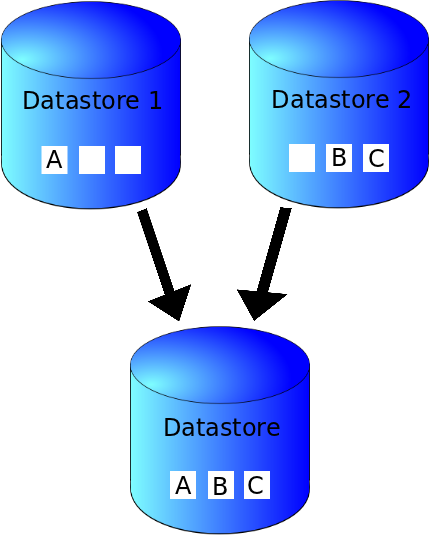
\includegraphics[height= 10cm, width=15cm]{project/images/data-sync}
  \caption{\textbf{IMAGE CAPTION}}
\end{figure}

 % adds the introduction page
\chapter{Especificación de requerimientos}
\section{Pila de producto}
Describa brevemente el producto en función del análisis de historias. Si es posible modifique la codificación de las historias para que el lector tenga un apoyo visual respecto a la estructura del sistema. Por ejemplo las historias correspondientes a los módulos de interfaz podrían codificarse UIXXX, mientras que las historias correspondientes a módulos de red podrían codificarse NTXXX. Explique en esta sección la lógica detrás de la codificación usada.

\subsection{Requerimientos funcionales del sistema}

%% PILA DE PRODUCTO %%
\begin{longtable}{|l||p{7cm}|l|l|}

\multicolumn{4}{c}{Pila general del producto}\\
\hline\hline
\textbf{Código} & \textbf{Descripción} & \textbf{Prioridad} & \textbf{Inserción}\\
\hline
\endfirsthead
\textbf{Código} & \textbf{Descripción} & \textbf{Prioridad} & \textbf{Inserción}\\
\hline\hline
\endhead

\textbf{RFXXX} & 
Descripción de la funcionalidad que representa la historia, lo más detallado posible & Alta & Original\\

\textbf{RF001} & Una historia original & Alta & Original \\

\color{ForestGreen}
\textbf{RF002} & Una historia nueva en este sprint & Media & Sprint 1 \\

\color{Mahogany}
\textbf{RF003} & Una historia eliminada & Baja & Original \\
\hline

\caption{\color{ForestGreen}VERDE: Historias agregadas en esta iteración. \color{Mahogany}ROJO: Historias eliminadas.}
\label{ProductBacklog}

\end{longtable}

\subsection{Bitácora de cambios}
Debe resumir en esta sección las decisiones que llevaron a la creación de nuevas historias, o la eliminación de historias ya analizadas. 

\section{Producto Mínimo Viable de la iteración X}

\subsection{Alcance del PMV}
Describa en esta sección el alcance que se proyectó para el PMV de esta iteración. Tome en cuenta que los PMV son incrementales, por lo que debe explicar cómo esta iteración aumentó la funcionalidad del PMV pasado.

\subsection{Pila de trabajo de la iteración X}

%% PILA DEL SPRINT (ITERACIÓN) %%

\begin{longtable}{|l||c|c|p{7cm}|l|c|}

\multicolumn{5}{c}{Pila de la \textbf{iteración X} }\\
\hline\hline
\textbf{Código} & \textbf{CE} & \textbf{CR} & \textbf{Responsables} & \textbf{Finalización}& \\
\hline
\endfirsthead
\textbf{Código} & \textbf{CE} & \textbf{CR} & \textbf{Responsables} & \textbf{Finalización} & \\
\hline\hline
\endhead

\textbf{RF001} & 3 & 3 & Responsable A, Responsable B & 2017/08/14 & $\square$\\

\color{ForestGreen}
\textbf{RF002} & 2 & 4 & Responsable A, Responsable B & 2017/08/25 & $\square$\\

% IMPORTANTE: La casilla de verificación para el Product Owner no debe incluirse en las historias eliminadas ni en las historias inconclusas. Solamente en aquellas que se lograron terminar en el Sprint
\color{Mahogany}
\textbf{RF003} & 5 & - & Responsable A, Responsable B & N/A &  \\
\hline

\caption{Pila de la Iteración X. \textbf{CE:} Carga Estimada, \textbf{CR:} Carga Real.}
\label{SprintBacklog}


\end{longtable}
 % Especificación de requerimientos
\chapter{Arquitectura del sistema}
\section{Diseño general del sistema}

Descripción en prosa del diseño del sistema. Resalte cualquier detalle que considere de importancia para la comprensión del diseño.

\subsection{Diagrama de clases}
Añada una imagen con el diagrama de clases del sistema,  preferiblemente desarrollado en DIA. Introdúzcala con un párrafo breve que enlace el diagrama con la descripción en prosa del encabezado de sección. Se recomienda que el diagrama se diseñe de forma que calce bien en una página vertical, de forma que se facilite su lectura. Recuerde hacer referencia a su diagrama de clases usando la referencia correcta. Por ejemplo, en la Figura \ref{DiagramaClases} se encuentra el diagrama de clases.
\begin{figure}[H]
  \centering
    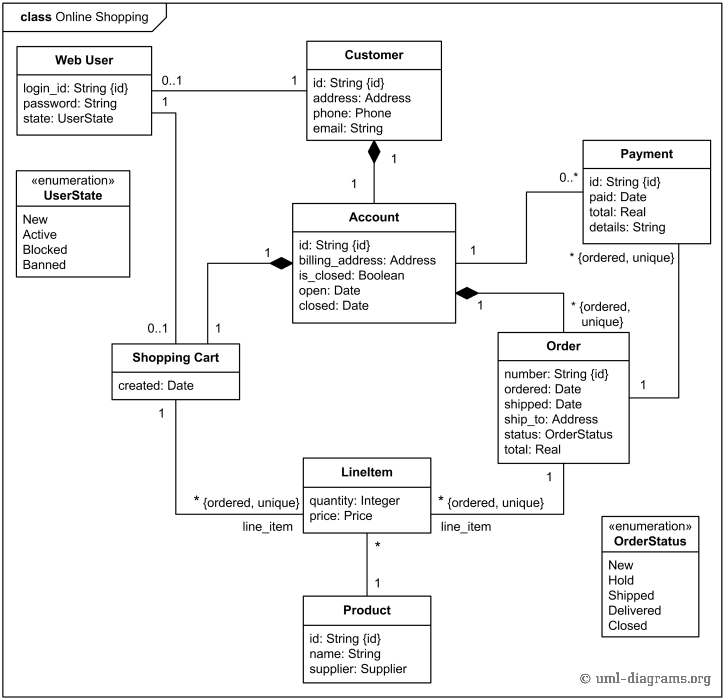
\includegraphics[ width=15cm]{project/images/class-example-online-shopping-domain.png}
  \caption{\textbf{IMAGE CAPTION}}
  \label{DiagramaClases}
\end{figure}

\subsection{Estrategias de diseño}
Describa en esta sección la aplicación de patrones de diseño identificados para su sistema. Incluya en la descripción los problemas detectados que se resolvieron por medio de la implementación del patrón. Adicionalmente describa la forma en que se adaptaron los patrones para que funcionaran correctamente con su sistema.

 % Diseño del sistema
\chapter{Prototypos de interfaz}
En este capítulo adjunte y describa los prototipos de la interfaz para su aplicación. Procure hacer referencia al diseño de interacción y diseño para la usabilidad presentes en su aplicación.
Si su aplicación tiene propiedades de accesibilidad para un público con necesidades especiales, por favor describa las estrategias usadas en esta sección.

\section{Prototipos de la funcionalidad X}
Recuerde poner un texto introductorio breve para cada sección.
\vspace{2cm}
\begin{figure}[H]
  \centering
    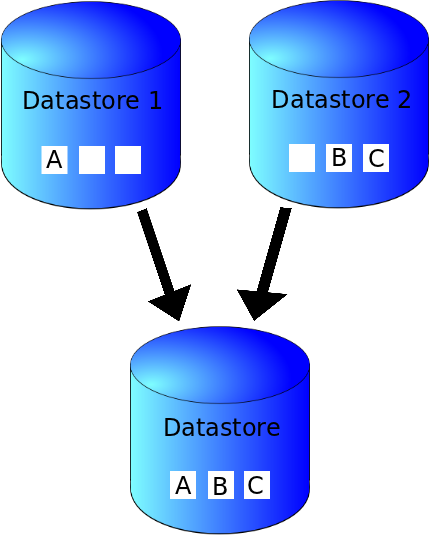
\includegraphics[height= 11cm, width=17cm]{project/images/data-sync}
\end{figure}
\newpage
\begin{figure}[H]
  \centering
    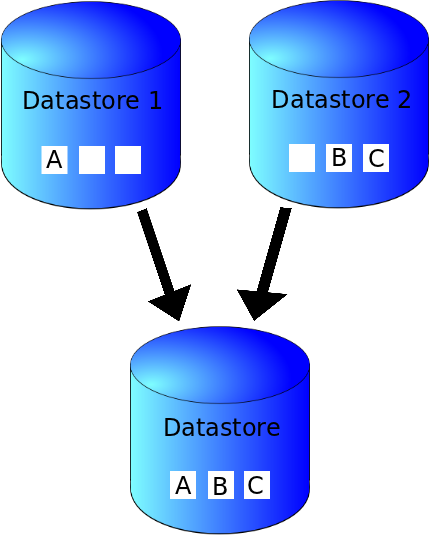
\includegraphics[height= 11cm, width=17cm]{project/images/data-sync}
\end{figure}
\vspace{1cm}

\section{Prototipos de la funcionalidad Y}
No olvide referenciar las imágenes en el texto usando \emph{label} y \emph{ref}.

\begin{figure}[H]
  \centering
    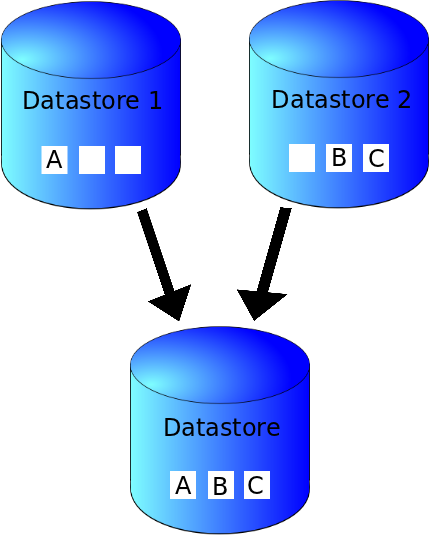
\includegraphics[height= 11cm, width=17cm]{project/images/data-sync}
\end{figure} % Prototipos de interfaz de usuario
\chapter{Control de calidad}
Introduzca en esta sección la estrategia utilizada para el control de calidad del producto. Incluya los miembros del equipo que participaron del proceso de control de calidad.
\section{Pruebas Internas}
Introduzca esta sección indicando cuántos scripts de pruebas se hicieron para el sistema propio. Indique cualquier detalle que crea necesario para que se entiendan los scripts de pruebas correctamente. Recuerde referencias los diferentes scripts usando las etiquetas y el \ref{TestSctipt1} correspondiente

\subsection{Guiones de pruebas internas}
\begin{longtable}{ | p{2cm} | p{3cm} | p{4cm} | p{4cm} | c |}
      \hline
      \textbf{Historias} & \textbf{Descripción} & \textbf{Resultado Esperado} & \textbf{Resultado Obtenido} & \textbf{Condición}\\
      \hline
      RF001 y RF003 & AAAA & BBBB & CCCC & \color{ForestGreen}PASÓ\\
      \hline
      RF002 y RF005 & AAAA & BBBB & CCCC & \color{Mahogany}FALLÓ\\
      \hline
      
      \caption{Descripción rápida del guión de pruebas}
      \label{TestScript1}
\end{longtable}

\begin{longtable}{ | p{2cm} | p{3cm} | p{4cm} | p{4cm} | c |}
      \hline
      \textbf{Historias} & \textbf{Descripción} & \textbf{Resultado Esperado} & \textbf{Resultado Obtenido} & \textbf{Condición}\\
      \hline
      RF001 y RF003 & AAAA & BBBB & CCCC & \color{ForestGreen}PASÓ\\
      \hline
      RF002 y RF005 & AAAA & BBBB & CCCC & \color{Mahogany}FALLÓ\\
      \hline
      
      \caption{Descripción rápida del otro guión de pruebas. Note que pueden haber varios guiones para la misma iteración.}
      \label{TestScript1}
\end{longtable}

\section{Pruebas Externas}
Introduzca en esta sección los guiones de pruebas que el otro equipo le aplicó a su sistema. Describa cada guión de pruebas y resuma el resultado general de las pruebas de su sistema. 

\subsection{Guiones de pruebas externas}
Incluya aquí los guiones de pruebas externas. Note que los guiones que debe incorporar son los que se aplicaron a su sistema. Estos debieron haberse entregado por el equipo de control cruzado oportunamente.

\begin{longtable}{ | p{2cm} | p{3cm} | p{4cm} | p{4cm} | c |}
      \hline
      \textbf{Historias} & \textbf{Descripción} & \textbf{Resultado Esperado} & \textbf{Resultado Obtenido} & \textbf{Condición}\\
      \hline
      RF001 y RF003 & AAAA & BBBB & CCCC & \color{ForestGreen}PASÓ\\
      \hline
      RF002 y RF005 & AAAA & BBBB & CCCC & \color{Mahogany}FALLÓ\\
      \hline
      
      \caption{Descripción rápida del guión de pruebas}
      \label{TestScript1}
\end{longtable} % Pruebas
\chapter{Capturas de pantalla}
En este capítulo puede mostrar capturas del sistema para que quede registro del avance del producto. Esta sección es opcional.
\section{Capturas de la funcionalidad X}
Recuerde poner un texto introductorio breve para cada sección.
\vspace{2cm}
\begin{figure}[H]
  \centering
    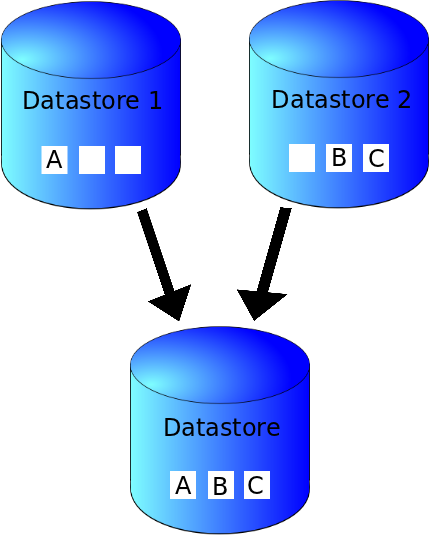
\includegraphics[height= 11cm, width=17cm]{project/images/data-sync}
\end{figure}
\newpage
\begin{figure}[H]
  \centering
    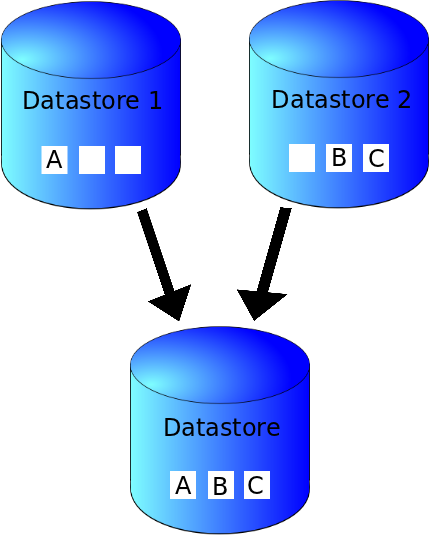
\includegraphics[height= 11cm, width=17cm]{project/images/data-sync}
\end{figure}
\vspace{1cm}

\section{Capturas de la funcionalidad Y}
No olvide referenciar las imágenes en el texto usando \emph{label} y \emph{ref}.

\begin{figure}[H]
  \centering
    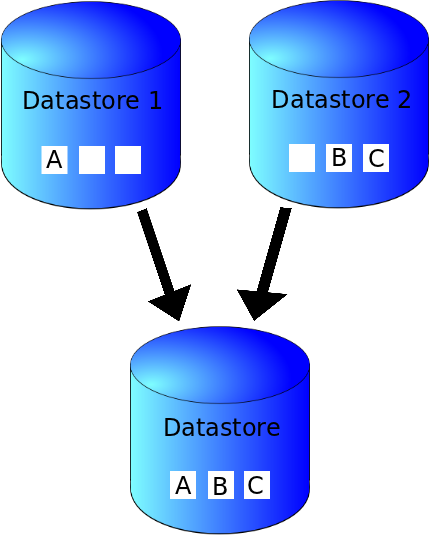
\includegraphics[height= 11cm, width=17cm]{project/images/data-sync}
\end{figure} % [OPCIONAL] Capturas de pantalla
\chapter{Conclusiones y trabajo futuro}
\section{Conclusiones}
\paragraph{}WRITE HERE.
\section{Problemáticas y limitaciones}
Recuerde que sólo debe registrar aquellas problemáticas que el sistema TIENE, no debe mencionar problemas que aparecieron durante el desarrollo, pero que se resolvieron adecuadamente.
Considere como problemáticas errores o comportamientos indeseables que el sistema tiene. Por ejemplo fugas de memoria, puntos en los que el sistema se cuelga, etc...
Limitaciones por el otro lado, son cosas que el sistema NO puede hacer, ya sea por diseño o por que se quería incluir pero no fue posible. Por ejemplo la falta de multijugador por Internet es una limitación, también liste aquí las plataformas para las cuales el sistema está diseñado (sistema operativo, requerimientos mínimos, resolución recomendada, etc...).

\section{Trabajo futuro}
Describa en esta sección qué considera que puede mejorarse en el futuro para este proyecto. 


%%Texto explicativo, no debe aparecer en el documento final
\section{NOTAS SOBRE LAS REFERENCIAS BIBLIOGRÁFICAS}
En el archivo references.bib puede agregar las fuentes bibliográficas usadas en el documento en formato \emph{bibtex}.
Puede incluir fuentes que no citó en el archivo de referencias. Aquellas que no citó automáticamente serán omitidas en la lista de referencias.
Para citar una referencia en el texto debe usar el comando \emph{cite}. 

Por ejemplo el artículo de Dean se cita usando \cite{dean2003}. 
Note cómo los libros de Ortíz y Sánchez no salen en las referencias. 

\emph{Procure eliminar esta sección de su documento}
%%Aquí termina el texto explicativo % Conclusiones del informe


\bibliographystyle{apacite}
\bibliography{project/references.bib} % Referencias bibliográficas

\end{document}